\section{PL Condition and Coordinate Descent}

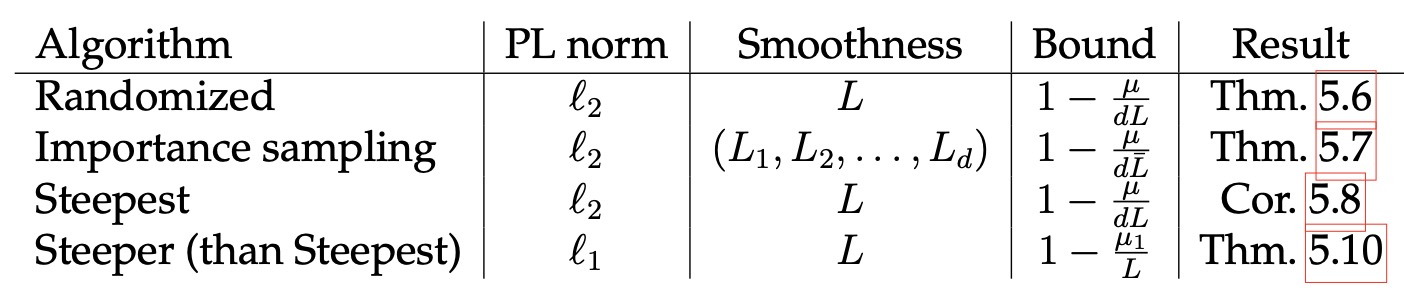
\includegraphics[width=\linewidth]{imgs/CGD.jpg}

\subsection{PL Condition}

\textbf{Definitions}:
\begin{enumerate}
    \item \textbf{Polyak-Lojasiewicz condition}: we say $f$ satisfies PL condition if $\frac{1}{2}\|\nabla f(x)\|^2 \ge \mu (f(x) - f(x^*))$.
    \item \textbf{Strong convexity w.r.t. $\|\cdot\|_1$}: $f(y) \ge f(x) + \nabla f(x)^\top (y-x) + \frac{\mu}{2}\|y-x\|_1^2$.
\end{enumerate}

\textbf{Properties}:
\begin{enumerate}
    \item \textbf{PL condition is weaker than strong convexity}: (5.2) if $f$ is $\mu$-strongly convex, then $f$ satisfies PL condition for the same $\mu$. Proof: by strong convexity, $f(x^*) - f(x) \ge \|\nabla f(x)\| \|y-x\| + \frac{\mu}{2} \|y-x\|^2 \ge -\frac{1}{2\mu}\|\nabla f(x)\|^2$.
    \item \textbf{PL condition is strictly weaker than strong convexity}: $f(x_1, x_2) = x_1^2$ is not strongly convex, but satisfies PL condition.
    \item \textbf{Smooth functions satisfying PL condition can be solved by GD in $O(\log(\frac{1}{\epsilon}))$}: for such functions, we have $f(x_T) - f(x^*) \le (1-\frac{\mu}{L})^T (f(x_0) - f(x^*))$. Proof: by sufficient descrease of $L$-smoothness, we have $f(x_{t+1}) \le f(x_t) - \frac{1}{2L}\|\nabla f(x_t)\|^2$. By PL condition, this means $f(x_{t+1}) \le f(x_t) - \frac{\mu}{L} (f(x_t) - f(x^*))$, which implies $f(x_{t+1}) - f(x^*) \le (1-\frac{\mu}{L}) (f(x_t) - f(x^*))$.
    \item \textbf{Strong convexity w.r.t. $\|\cdot\|_1$ and $\|\cdot\|_2$}: if $f$ is $\mu$-strongly convex w.r.t. $\|\cdot\|_1$, then $f$ is also $\mu$-strongly convex w.r.t. $\|\cdot\|_2$; if $f$ is $\mu$-strongly convex w.r.t. $\|\cdot\|_2$, then $f$ is $\mu / d$-strongly convex w.r.t. $\|\cdot\|_1$. Proof: use $\|x\|_1 \ge \|x\|_2$ and $\|x\|_2 \ge \frac{1}{\sqrt{d}}\|x\|_1$.
    \item \textbf{Strong convexity w.r.t. $\|\cdot\|_1$ implies PL condition w.r.t. $\|\cdot\|_\infty$}: (5.9) if $f$ has strong convexity w.r.t. $\|\cdot\|_1$, then $\frac{1}{2}\|\nabla f(x)\|_\infty^2 \ge \mu (f(x) - f(x^*))$. Proof: simply use $\nabla f(x)^\top (y-x) \le \|\nabla f(x)\|_\infty \|y-x\|_1$ in (5.2) instead.
\end{enumerate}


\subsection{Coordinate Descent}

\textbf{Coordinate-wise smoothness}: $f$ is called coordinate-wise smooth with parameter $L = (L_1, \dots, L_d)$ if for every coordinate $i$ we have $f(x + \lambda e_i) \le f(x) + \lambda \nabla_i f(x) + \frac{L_i}{2} \lambda^2$.

\textbf{Coordinate Descent Algorithm}: for each iteration $t$, choose an active coordinate $i \in [d]$, then do $x_{t+1} = x_t - \gamma_i \nabla_i f(x_i) e_i$.

\textbf{Sufficient decrease}: (5.5) with $\gamma_i = 1 / L_i$, we have $f(x_{i+1}) \le f(x_i) - \frac{1}{2L_i} |\nabla_i f(x_t)|^2$. Proof: plugging the update step into the definition of coordinate-wise smoothness immediately gives the result.

\textbf{Analysis for coordinate-wise smooth functions satisfying PL condition}:
\begin{enumerate}
    \item \textbf{Randomized coordinate descent}: (5.6) choose coordinate uniformly at random and set $\gamma_i = 1/L$ where $L = \max_i L_i$, the randomized coordinate descent gets $\E(f(x_T) - f(x^*)) \le (1-\frac{\mu}{d L})^T (f(x_0) - f(x^*))$. This means randomized coordinate descent is the same good as GD, as the number of iterations is $d$ times higher, but each iteration is $d$ times cheaper. Proof: by sufficient decrease of coordinate descent, $\E (f(x_{t+1}) \mid x_t) \le f(x_t) - \frac{1}{2L} \sum_{i=1}^d \frac{1}{d} |\nabla_i f(x_t)|^2 = f(x_t) - \frac{1}{2dL} \|\nabla f(x_t)\|^2$. By PL condition, this means $\E (f(x_{t+1}) \mid x_t) \le f(x_t) - \frac{\mu}{dL}(f(x_t) - f(x^*))$, which implies $\E(f(x_{t+1}) - f(x^*) \mid x_t) \le (1-\frac{\mu}{dL})(f(x_t) - f(x^*))$. This means $\E(f(x_{t+1}) - f(x^*)) \le (1-\frac{\mu}{dL})\E(f(x_t) - f(x^*))$.
    \item \textbf{Importance sampling}: (5.7) choose coordinate $i$ with probability $\frac{L_i}{\sum_j L_j}$ and define $\bar{L} = \frac{1}{d}\sum_{i=1}^d L_i$, we have $\E(f(x_T) - f(x^*)) \le (1-\frac{\mu}{d\bar{L}})^T (f(x_0) - f(x^*))$. Note how randomized coordinate descent for $L$-smooth functions is a special case of this result. Proof: $\E (f(x_{t+1}) \mid x_t) \le f(x_t) - \frac{1}{2} \sum_{i=1}^d \frac{L_i}{\sum_j L_j} \frac{1}{L_i} |\nabla_i f(x_t)|^2 = f(x_t) - \frac{1}{2d\bar{L}}\sum_i |\nabla_i f(x_t)|^2$. The rest is the same to (5.6).
    \item \textbf{Steepest coordinate descent}: (5.8) choose coordinate $i = \argmax_i |\nabla_i f(x_t)|$, we have $f(x_T) - f(x^*) \le (1-\frac{\mu}{d L})^T (f(x_0) - f(x^*))$. Proof: simply remove the expectation and use maximum is greater than average.
    \item \textbf{Steepest descent for strong convexity w.r.t. $\|\cdot\|_1$}: (5.10) if $f$ is $\mu_1$-strongly convex w.r.t. $\|\cdot\|_1$, then with $\gamma_i = 1/L$, steepest descent gives $f(x_T) - f(x^*) \le (1- \frac{\mu_1}{L})^T (f(x_0) - f(x^*))$. Note that steepest descent has the same per iteration cost as GD, but the $\mu_1$ could be greater than the $L_2$ strong convexity parameter. Proof: by sufficient decrease and the update rule, $f(x_{t+1}) \le f(x_t) - \frac{1}{2L}\|\nabla f(x_t)\|_\infty^2$. By the PL condition w.r.t. $\|\cdot\|_\infty$, this means $f(x_{t+1}) \le f(x_t) - \frac{\mu_1}{L} (f(x_t) - f(x^*))$ and thus $f(x_{t+1}) - f(x^*) \le (1- \frac{\mu_1}{L})(f(x_t) - f(x^*))$.
    \item \textbf{Greedy coordinate descent}: choose some coordinate, then do $x_{t+1} = \argmin_\lambda f(x_t + \lambda e_i)$, i.e., make the largest step possible. For differentiable convex functions, as the update can only be better than before, it does not compromise the analysis. For non-differentiable case, however, it may get stuck in non-optimal points. (5.11) Assume $f(x) = g(x) + h(x)$, where $h(x) = \sum_i h_i (x_i)$, $g$ is convex and differentiable and $h_i$ is convex, then if the greedy descent converges, it converges to the global minimum of $f$. Such $h$ is called \emph{separable}, which includes $L_1$ norm and squared $L_2$ norm. This means LASSO and ridge objectives are concrete cases. Proof: $f$ is the sum of convex functions, thus convex. Let $x$ be the converged point and $y$ be a near point. Thus, $\nabla_i g(x) (y_i - x_i) + h_i(y_i) - h_i(x_i) \ge 0$, since the algorithm converges. By first-order characterization, we have $f(y) - f(x) \ge \nabla g(x)^\top (y-x) + \sum_i (h_i(y_i) - h_i(x_i)) \ge 0$.
\end{enumerate}